\documentclass[a4paper, 12pt]{article}

\usepackage{wrapfig}
\usepackage{graphicx}
\usepackage{mathtext}
\usepackage{amsmath}
\usepackage{siunitx}
\usepackage{multirow}
\usepackage{rotating}

\usepackage[T1,T2A]{fontenc}

\usepackage[russian]{babel}

\graphicspath{{pictures/}}

\title{\begin{center}Лабораторная работа №1.4.1\end{center}
ИЗУЧЕНИЕ ЭКСПЕРИМЕНТАЛЬНЫХ ПОГРЕШНОСТЕЙ НА ПРИМЕРЕ ФИЗИЧЕСКОГО МАЯТНИКА}
\author{Гёлецян А.Г.}
\date{\today}

\begin{document}
    \pagenumbering{gobble}
    \maketitle
    \newpage
    \pagenumbering{arabic}

    \section{Введение}
    \textbf{Цель работы:}
    \begin{itemize}
     \item проверить справедливость формулы для периода колебаний физического маятника и определить значение ускорения свободного падения
     \item убедиться в справедливости теоремы Гюйгенса об обратимости
    точек опоры и центра качания маятника
    \end{itemize}

    \vspace{1cm}

    \textbf{В работе используются: }
    \begin{itemize}
        \item металлический стержень
        \item опорная призма
        \item торцевые ключи
        \item закреплённая на стене консоль
        \item подставка с острой гранью для определения цента масс маятника
        \item секундомер
        \item линейки металлические длиной 30, 50 и 100 см
        \item штангенциркуль
        \item электронные весы
        \item математический маятник
    \end{itemize}

    \newpage

%     \begin{center}\textbf{Теория}\end{center}
    \section{Теория}
    \begin{wrapfigure}{l}{0.5\linewidth}
        \begin{center}
            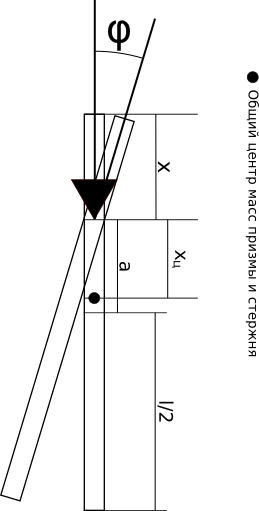
\includegraphics[scale=0.8]{gr.png}
            \caption{Схема установки}
        \end{center}
    \end{wrapfigure}

    Напишем уравнение движения системы

    \[-(m+M)gx_ц \sin{\varphi} = (I_m+I_M)\ddot{\varphi}\]

    где $m, I_m$ это масса и момент инерции призмы соответственно, а $M, I_M$ это масса и момент инерции стержня соответственно.

    Из теоремы Штайнера-Гюйгенса \[I_M=Ml^{2}/12+Ma^2\]
    В наших измерениях $m\approx M/11$, а расстояние центра масс призмы от оси качения составляет примерно $a_m=1.5см$. В измерениях минимальное значение $a$, которое использовалось в измерениях составляет $a_{min}=12.5см$. Таким образом оценим какая доля имеет момент инереции призмы в системе.
    \[\frac{I_m}{I_M}=\frac{m}{M}\frac{a_m^{2}}{a_{min}^{2}+\frac{l^{2}}{12}}\approx 0.02\%\]
    Так как эта величина на порядки меньше относительных погрешностей всех других измерении, мы имеем полное моральное право пренебрегать $I_m$ относительно $I_M$.
    \newline
    При приближении $\varphi\ll 1$ наше уравнение движения переходит в уравнение гармонического осцилятора, откуда можно легко получить формулу периода колебания маятника
    \begin{equation}
        T=2\pi \sqrt{\frac{\frac{l^{2}}{12}+a^{2}}{\beta x_ц g}}
    \end{equation}

    где $\beta=1+m/M$.

    \newpage

    \section{Ход работы}
    \paragraph{}
    Для начала измерим все статические величины.
    \vspace{0.5cm}
    \newline$l=(100.1\pm0.05)см$
    \newline$m=(76.3\pm0.1)г$
    \newline$M=(870.5\pm0.1)г$
    \vspace{0.5cm}

    \paragraph{}
    Чтобы понять сколько знаков нам хранить для $\beta$ для начала подсчитаем его погрешность
    \begin{equation}
        \Delta\beta=\sqrt{(\Delta m \frac{\partial \beta}{\partial m})^{2} +
                          (\Delta M \frac{\partial \beta}{\partial M})^{2}} =
                  \sqrt{(\frac{\Delta m}{M})^{2} + (\frac{\Delta M m}{M^{2}})^{2}} \approx 0.0001
    \end{equation}


    \paragraph{}
    Мы видим, что после запятой можем хранить 4 цифры, поэтому
    \[\beta=1.0877\pm0.0001\]

    \paragraph{}
    Для проведения серии измерении($a=const$) фиксируем призму в каком то положении $a$ и несколько раз($N=8$) измеряем время $n$ колебании. Обозначим это время $t$. Погрешность измерения $a$ равна $\Delta a=0.1см$, т.к. $a$ является разницой двух измерении с погреностью $0.05см$ ($a=l/2 - x$). Для краткости в работе указаны сразу $a$, без указания $x$. То же самое верно и для $x_ц$ ($\Delta x_ц = 0.1см$).
    \paragraph{}
    Период колебания считаем по формуле $T=t/n$, а случайную ошибку по формуле
    \[\Delta T_{случ} = \frac{1}{n} \sqrt{\frac{1}{N-1}\sum{(t_i - \bar{t})^{2}}}\]
    Систематическая ошибка $\Delta t_{сист}=0.02с$ (примерное время обновления экрана секундомера). Так как $T=t/n$, то $\Delta T_{сист}=\Delta t_{сист}/n$. Полная ошибкаha
    \[\Delta T = \sqrt{{\Delta T_{сист}}^{2} + {\Delta T_{случ}}^{2}}\]
    \newpage
    \paragraph{}
    В Таблице 1 приведены данные измерении. В Таблице 2 приведены периоды колебании с погрешностями. В Таблице 3 приведены расчетные значения $g$ и $\Delta g_{сист}$. Последняя считалось по аналогичной $(2)$ формуле.
    \vspace{1cm}
    \begin{table}[h!]
        \begin{center}

         \begin{tabular}{|c|c|c|c|c|c|c|c|c|}
            \hline
            \textbf{Серия} & \textbf{1} & \textbf{2} & \textbf{3} & \textbf{4} & \textbf{5} & \textbf{6} & \textbf{7} & \textbf{8}\\
            \hline
            \textbf{$a, см$} & 39.3 & 32.5 & 29.2 & 24.3 & 22.0 & 19.1 & 15.3 & 12.4\\
            \hline
            \textbf{$x_ц, см$} & 36.0 & 29.8 & 26.8 & 22.2 & 20.1 & 17.4 & 14.0 & 11.3\\
            \hline
            \textbf{$n$} & 20 & 20 & 20 & 10 & 10 & 20 & 20 & 20\\
            \hline
            \multicolumn{9}{c}{  } \\
            \hline
            № опыта & \multicolumn{8}{c|}{$t, с$} \\
            \hline
            1 & 31.30 & 30.69 & 30.63 & 15.43 & 15.59 & 31.94 & 33.76 & 36.03 \\
            2 & 31.21 & 30.61 & 30.62 & 15.39 & 15.55 & 31.98 & 33.69 & 35.97 \\
            3 & 31.25 & 30.70 & 30.63 & 15.43 & 15.58 & 31.89 & 33.65 & 35.94 \\
            4 & 31.28 & 30.64 & 30.57 & 15.41 & 15.66 & 31.98 & 33.73 & 36.00 \\
            5 & 31.30 & 30.61 & 30.64 & 15.46 & 15.60 & 31.95 & 33.72 & 35.96 \\
            6 & 31.27 & 30.68 & 30.61 & 15.40 & 15.67 & 31.97 & 33.73 & 35.94 \\
            7 & 31.27 & 30.70 & 30.53 & 15.48 & 15.71 & 31.94 & 33.77 & 35.98 \\
            8 & 31.26 & 30.70 & 30.62 & 15.40 & 15.65 & 32.03 & 33.68 & 35.98 \\
            \hline
         \end{tabular}
         \caption{Измерения времени $t$ для $n$ колебании}
        \end{center}

    \end{table}


    \begin{table}[h!]
        \begin{center}

         \begin{tabular}{|c|c|c|c|c|c|c|c|c|}
            \hline
            \textbf{$a, см$} & 39.3 & 32.5 & 29.2 & 24.3 & 22.0 & 19.1 & 15.3 & 12.4\\
            \hline
            \textbf{$T, с$} & 1.563 & 1.533 & 1.530  & 1.542 & 1.563 & 1.598 & 1.686 & 1.799\\
            \hline
            \textbf{$\Delta T, с$} & 0.002 & 0.002 & 0.002 & 0.004 & 0.006 & 0.002 & 0.002 & 0.002\\
            \hline
         \end{tabular}
         \caption{Периоды колебании для различных $a$}
        \end{center}

    \end{table}

    \begin{table}[h!]
        \begin{center}

         \begin{tabular}{|c|c|c|c|c|c|c|c|c|}
            \hline
            № опыта & \multicolumn{8}{c|}{$g, см/с^{2}$} \\
            \hline
            1 & 980 & 979 & 976 & 981 & 982 & 984 & 976 & 983 \\
            2 & 986 & 985 & 977 & 986 & 988 & 982 & 980 & 986 \\
            3 & 983 & 979 & 976 & 981 & 984 & 987 & 983 & 988 \\
            4 & 981 & 983 & 980 & 984 & 974 & 982 & 978 & 985 \\
            5 & 980 & 985 & 975 & 977 & 981 & 984 & 979 & 987 \\
            6 & 982 & 980 & 977 & 985 & 972 & 982 & 978 & 988 \\
            7 & 982 & 979 & 982 & 975 & 968 & 984 & 976 & 986 \\
            8 & 983 & 979 & 977 & 985 & 975 & 979 & 981 & 986 \\
            \hline
            \multicolumn{9}{c}{}\\
            \hline
            $\bar{g}, см/с^{2}$ & \multicolumn{8}{c|}{981}\\
            \hline
            $\Delta g_{случ}, см/с^{2}$ & \multicolumn{8}{c|}{4}\\
            \hline
            $\Delta g_{сист}, см/с^{2}$ &5 & 6 & 6 & 7 & 9 & 7 & 8 & 9\\
            \hline
         \end{tabular}
         \caption{Расчетные $g$ для каждого измерения}
        \end{center}

    \end{table}
    \newpage
    \subsection{$g$ методом усреднения}
    \paragraph{}
    Начнем подсчет результатов с подсчета $g$ методом усреднения.
    \[\bar{g}=981см/с^{2}, \Delta g_{случ}=4см/с^{2}\]
    \paragraph{}
    Для подсчета систематических ошибок воспользуемся формулой, аналогичной формуле $(2)$. Для оценки полной погрешности возмем $\Delta g_{сист}$ как средюю из Таблицы 3.
    \[\Delta g_{сист} \approx 7см/с^{2}, \Delta g = \sqrt{{\Delta g_{сист}}^{2} + {\Delta g_{случ}}^{2}}\approx 8см/с^{2}\]
    \paragraph{}
    Финальный ответ.
    \[g=(981\pm8)см/с^{2}, {\varepsilon}_g\approx 0.8\%\]

    \subsection{Минимум $T(a)$}
    \paragraph{}
    Из графика на Рис. 2 видно, что зависимость $T(a)$ имеет минимум, и он находится около $a=28см$. Согласно приближенной формуле, где не учитывается влияние массы призмы на положение общего центра масс, минимум можно найти решив уравнение
    \[\frac{d}{da}(a+\frac{l^2}{12a})=0 \implies a=\frac{l}{2\sqrt{3}}\approx 29см\]
    так как количество вблизи минимума у нас не так уж и велико, и выражение для минимума не учитывает влияние массы призмы, можно удтверждать что эксперимент соответствует теории.

    \subsection{$g$ методом МНК}
    Если ввести обозначения $u=T^2x_ц$ и $v=a^2$, то формулу периода можно переписать как
    \[u=\frac{4\pi^2}{g\beta}(v+\frac{l^2}{12})\]
    Видим что между $u$ и $v$ есть линейная связь, о чем и свидетельствуют графики на Рис. 3 и 4.
    \[\Delta v = 2a\Delta a, \Delta u = \sqrt{(T^2\Delta x_ц)^2 + (2Tx_ц\Delta T)^2}\]
    Составим таблицу данных графика 3 (Рис. 4).
    \begin{table}[h!]
        \begin{center}

         \begin{tabular}{|c|c|c|c|c|c|c|c|c|}
            \hline
            \textbf{$u, с^{2}см$} & 88.0 & 70.1 & 62.8 & 52.8 & 49.1 & 44.4 & 39.8 & 36.6\\
            \hline
            \textbf{$\Delta u,с^{2}см$} & 0.3 & 0.3 & 0.3 & 0.4 & 0.4 & 0.3 & 0.3 & 0.3\\
            \hline
            \textbf{$v, см^{2}$} & 1541 & 1053 &  850 &  588 &  482 &  363 &  233 &  153\\
            \hline
            \textbf{$\Delta v, см^{2}$} & 8 & 6 & 6 & 5 & 4 & 4 & 3 & 2\\
            \hline
         \end{tabular}
         \caption{Значения $u$, $\Delta u$, $v$, $\Delta v$}
        \end{center}

    \end{table}
    \newline
    Методом наименьших квадратов находим коэффиценты $k$ и $b$ для уравнения $u=kx+b$, где $k=\frac{4\pi^2}{g\beta}$ а $b=k\frac{l^2}{12}$. Расчитаем также случайные ошибки $k$ и $b$, которые появляются из за МНК (для краткости оставим формулы расчета погрешностей коэффицентов МНК).
    \[k=(0.0370\pm0.0002)с^2/см\]
    \[b=(100.4\pm0.2)с^2см\]
    Теперь рассчитаем $g$ и $l$ из коэффицентов.
    \[g=\frac{4\pi^2}{k\beta}, \Delta g = g\sqrt{\left(\frac{\Delta k}{k}\right)^2 + \left(\frac{\Delta \beta}{\beta}\right)^2}\]
    \[l=\sqrt{\frac{12b}{k}}, \Delta l = l\sqrt{\left(\frac{\Delta b}{2b}\right)^2+\left(\frac{\Delta k}{2k}\right)^2}\]
    Подставив числа получаем
    \[g=(981\pm9)см/с^2, l=(100.4\pm0.5)см\]

    \subsection{Опыт с приведенной длиной маятника}
    \paragraph{}
    Если в формуле $(1)$ ввести обозначение $l_{пр}=\frac{l^{2}/{12}+a^{2}}{\beta x_ц}$, то формулу периода можно переписать как
    \[T=2\pi\sqrt{\frac{l_{пр}}{g}}\]
    Это означает, что период математического маятника с длиной $l_{пр}$ будет совпадать с периодом физического маятника. Проверим это на опыте.
    \paragraph{}
    Физический маятник имеет конфигурацию 1 (см. Таблицу 1) \newline $a=39.3см,x_ц=36.0см$. Подставив числа получаем $l_{пр}=60.8см$. Теперь измерим период математического маятника с этой длиной.

    \begin{table}[h!]
        \begin{center}

         \begin{tabular}{|c|c|c|c|c|c|}
            \hline
            \textbf{$t, с$} & 31.50 & 31.48 & 31.50 & 31.47 & 31.45\\
            \hline
            \textbf{$T,с$} & 1.575 & 1.574 & 1.575 & 1.574 & 1.573\\
            \hline
         \end{tabular}
         \caption{Периоды колебания математического маятника $(n=20)$}
        \end{center}

    \end{table}
    \paragraph{}
    Из этих данных получаем ${T_{мат}}=1.574с$. Период физического маятника $T_{физ}=(1.563\pm0.002)с$. Теперь подсчитаем погрешность $T_{мат}$ и проверим равенство этих периодов.
    \[\Delta  T_{мат}^{сист} = \Delta l_{пр}\frac{T_{мат}}{2l} \approx 0.013с\]
    \paragraph{}
    В расчете $\Delta l_{пр}=1см$, т.к. установка длины маятника было довольно не точным в связи с шаровидностю груза и прогиба линейки. Как видим в пределах погрешности эти периоды совпадают, поэтому в пределах погрешности формула приведенной длины маятника работает.
    \paragraph{}
    Теперь проделаем опыт по переворачиванию маятника относительно точки с расстоянием $l_{пр}$.

    \begin{table}[h!]
        \begin{center}

         \begin{tabular}{|c|c|c|c|c|c|}
            \hline
            \textbf{$t, с$} & 31.34 & 31.28 & 31.25 & 31.24 & 31.24\\
            \hline
            \textbf{$T,с$} & 1.567 & 1.564 & 1.563 & 1.562 & 1.562\\
            \hline
         \end{tabular}
         \caption{Периоды колебания перевернутого маятника $(n=20)$}
        \end{center}

    \end{table}
    \paragraph{}
    Получаем период $T_{пер}=1.564с$, что в пределах погрешности $T_{физ}$. Еще раз удтверждаемся, что формула приведенной длины работает.

    \section{Заключение}
    \paragraph{}
    Как видим в пределах погрешности ускорение свободного падения, расчетная длина стержня совпадают с реальными значениями, а формулы периода маятника и теорема об обратимости центра качения и точки опоры прпвдивы в пределах погрешности.
    \newpage
    \begin{sidewaysfigure}
        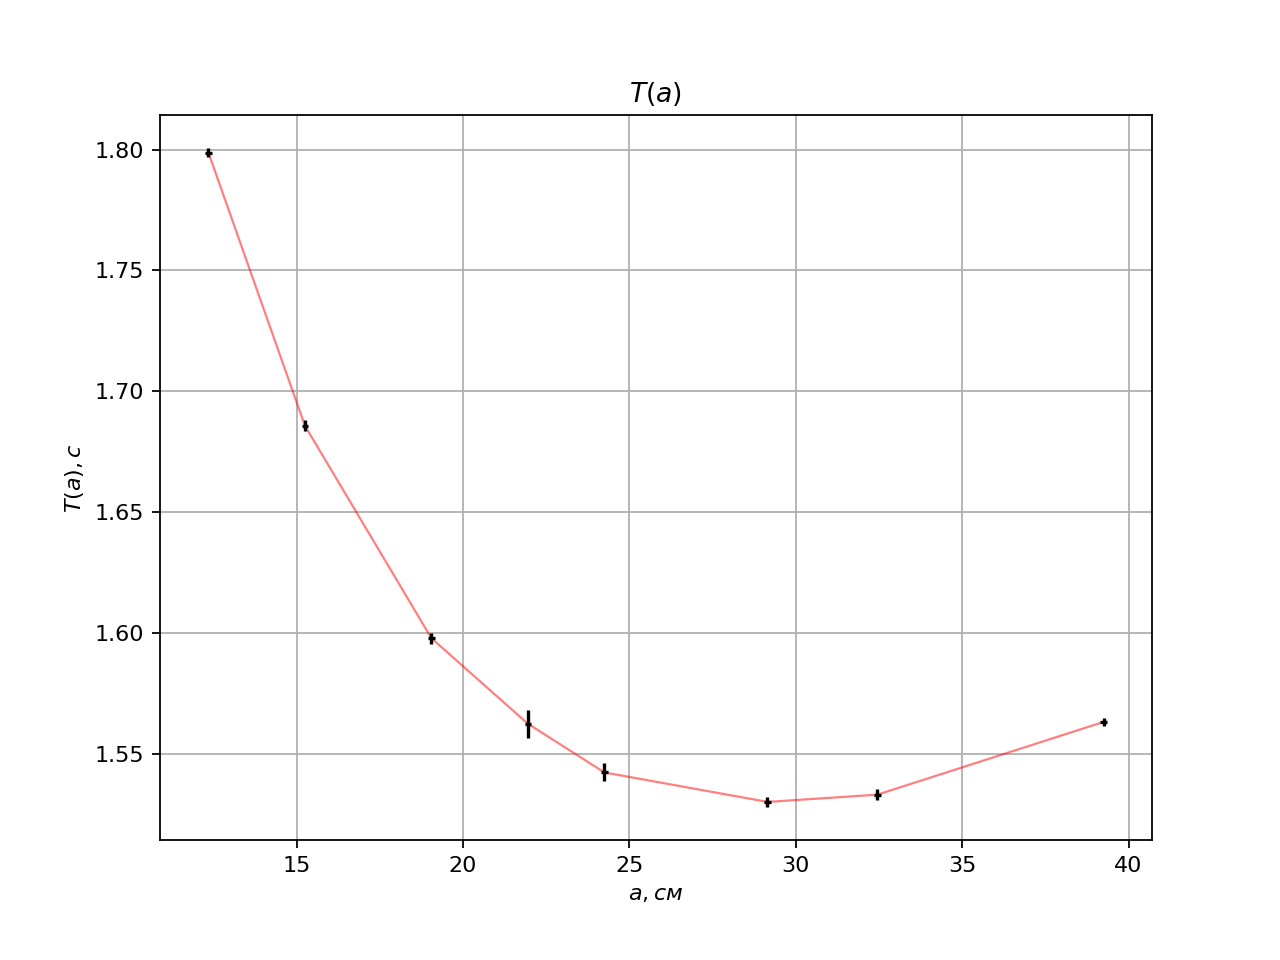
\includegraphics[scale=1.2]{plot1.png}
        \caption{График зависимости $T(a)$}
    \end{sidewaysfigure}

    \newpage
    \begin{sidewaysfigure}
        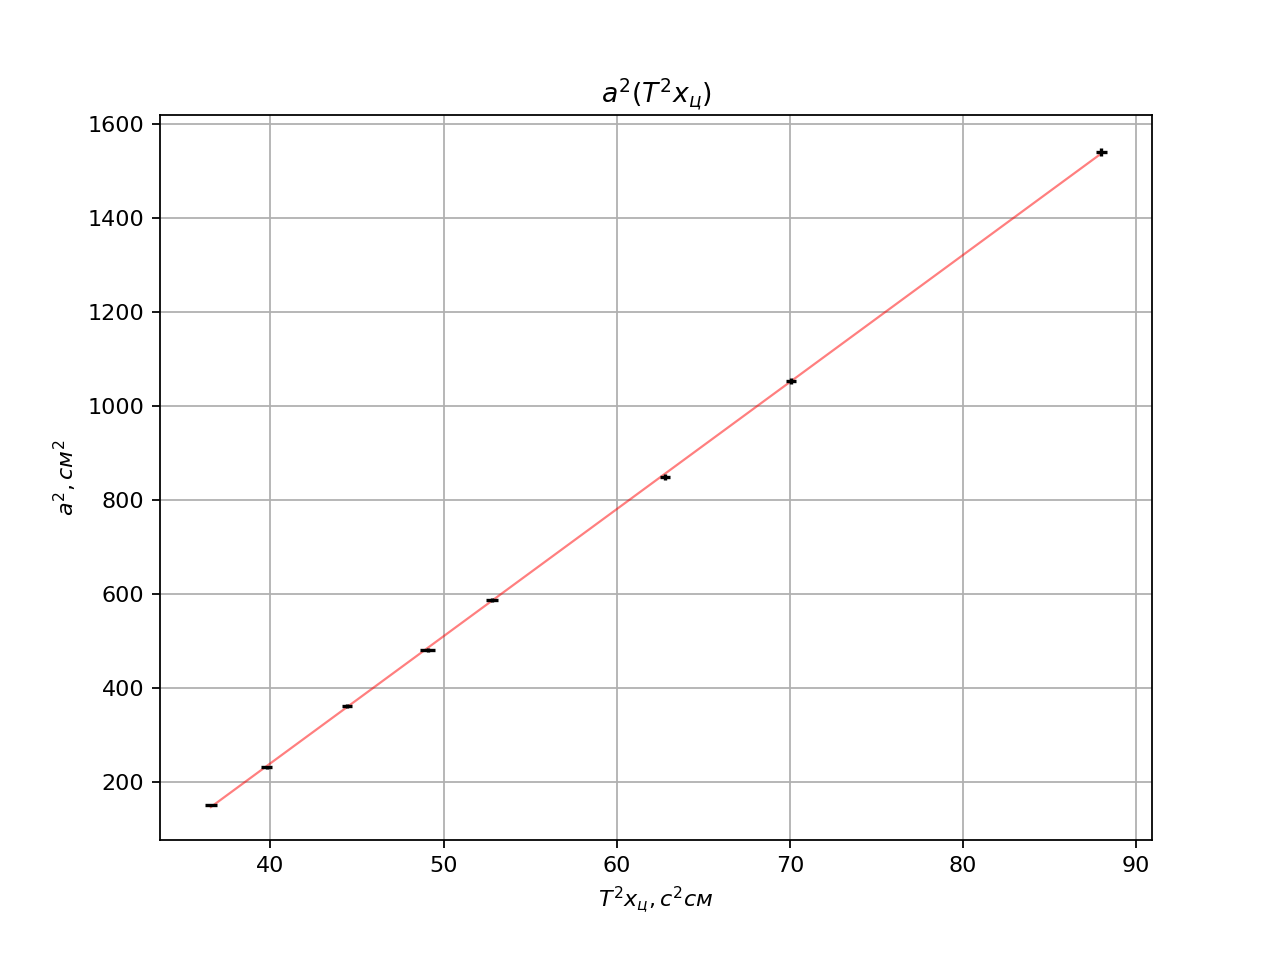
\includegraphics[scale=1.2]{plot2.png}
        \caption{График зависимости $a^2(T^2x_ц)$}
    \end{sidewaysfigure}

    \newpage
    \begin{sidewaysfigure}
        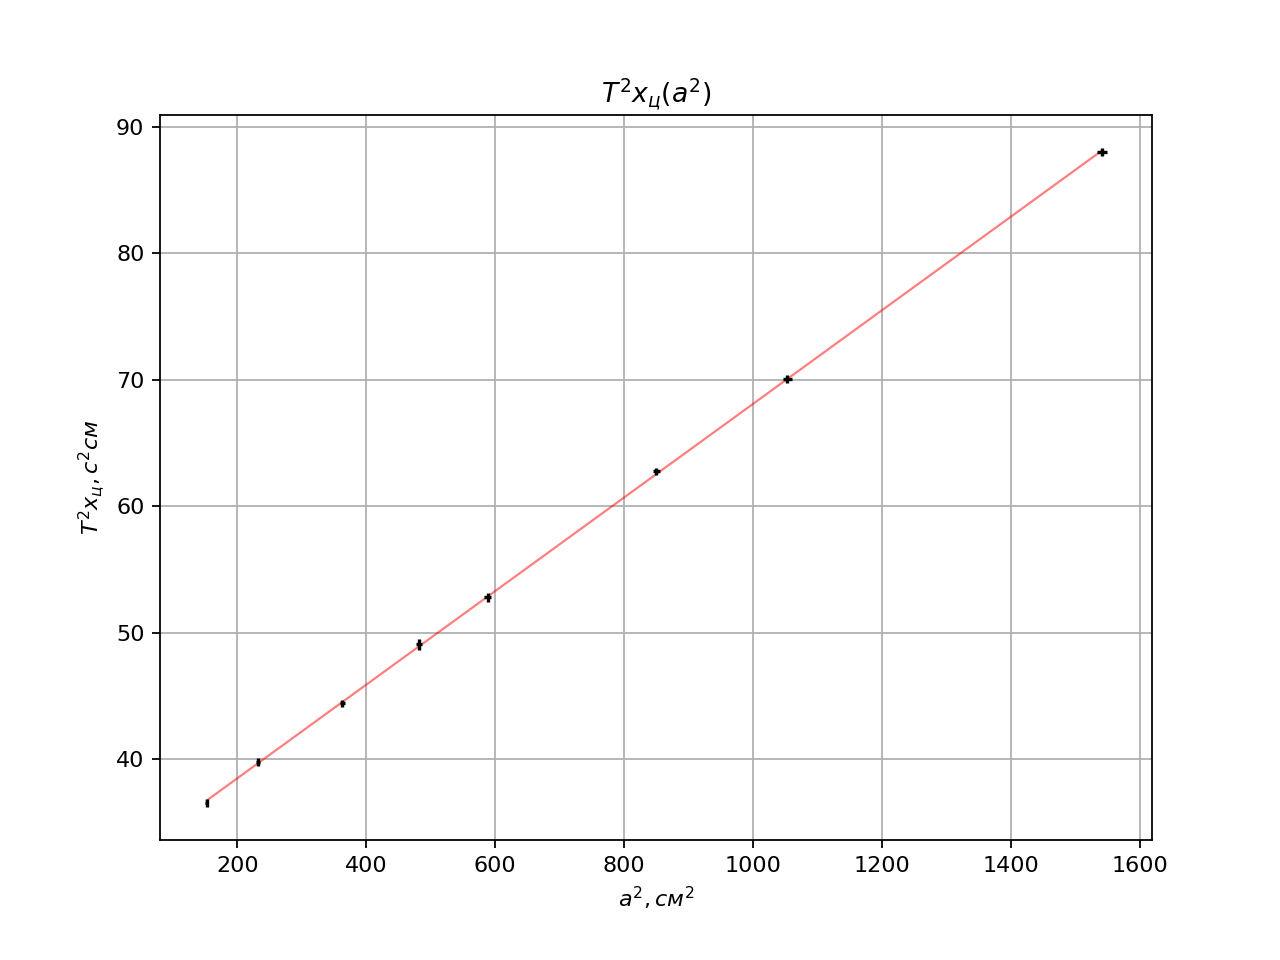
\includegraphics[scale=1.2]{plot3.png}
        \caption{График зависимости $T^2x_ц(a^2)$}
    \end{sidewaysfigure}
\end{document}

